\definecolor{myLightGray}{RGB}{191,191,191}
\definecolor{myGray}{RGB}{160,160,160}
\definecolor{myDarkGray}{RGB}{144,144,144}
\definecolor{myDarkRed}{RGB}{167,114,115}
\definecolor{myRed}{RGB}{255,58,70}
\definecolor{myGreen}{RGB}{0,255,71}

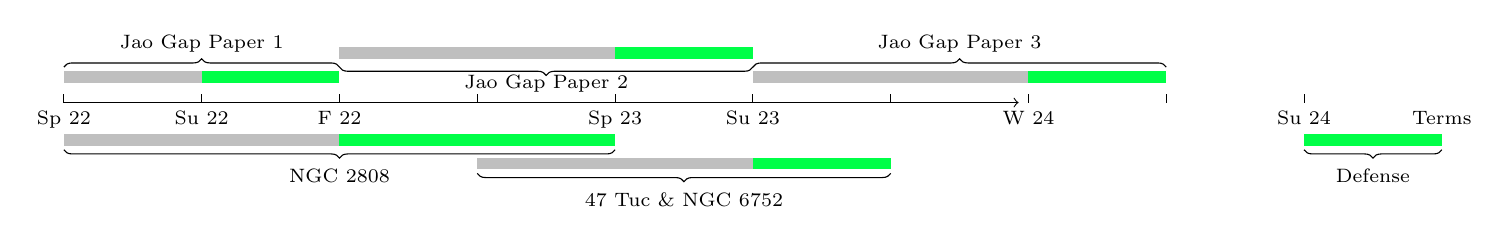
\begin{tikzpicture}[%
    every node/.style={
        font=\scriptsize,
        % Better alignment, see https://tex.stackexchange.com/questions/315075
        text height=1ex,
        text depth=.25ex,
    },
]
% draw horizontal line   
\draw[->] (0,0) -- (\textwidth,0);

% draw vertical lines
\foreach \x in {0,1,...,9}{
    \draw (1.75*\x cm,3pt) -- (1.75*\x cm,0pt);
}

% place axis labels
\node[anchor=north] at (1.75*0,0) {Sp 22};
\node[anchor=north] at (1.75*1,0) {Su 22};
\node[anchor=north] at (1.75*2,0) {F 22};
\node[anchor=north] at (1.75*4,0) {Sp 23};
\node[anchor=north] at (1.75*5,0) {Su 23};
\node[anchor=north] at (1.75*7,0) {W 24};
\node[anchor=north] at (1.75*9,0) {Su 24};
\node[anchor=north] at (1.75*10,0) {Terms};

% draw scale above
\fill[myLightGray] (1.75*0,0.25) rectangle (1.75*1,0.4);
\fill[myGreen]  (1.75*1,0.25) rectangle (1.75*2,0.4);

\fill[myLightGray] (1.75*2,0.55) rectangle (1.75*3,0.7);
\fill[myLightGray] (1.75*3,0.55) rectangle (1.75*4,0.7);
\fill[myGreen]  (1.75*4,0.55) rectangle (1.75*5,0.7);

\fill[myLightGray] (1.75*5,0.25) rectangle (1.75*6,0.4);
\fill[myLightGray] (1.75*6,0.25) rectangle (1.75*7,0.4);
\fill[myGreen]  (1.75*7,0.25) rectangle (1.75*8,0.4);
% draw scale below
\fill[myLightGray] (1.75*0,-0.4) rectangle (1.75*1,-0.55);
\fill[myLightGray] (1.75*1,-0.4) rectangle (1.75*2,-0.55);
\fill[myGreen] (1.75*2,-0.4) rectangle (1.75*3,-0.55);
\fill[myGreen] (1.75*3,-0.4) rectangle (1.75*4,-0.55);

\fill[myLightGray] (1.75*3,-0.7) rectangle (1.75*4,-0.85);
\fill[myLightGray] (1.75*4,-0.7) rectangle (1.75*5,-0.85);
\fill[myGreen] (1.75*5,-0.7) rectangle (1.75*6,-0.85);


\fill[myGreen] (1.75*9,-0.4) rectangle (1.75*10,-0.55);

% draw curly braces and add their labels
\draw[decorate,decoration={brace,amplitude=3pt}] (0,0.45) -- (1.75*2,0.45)
    node[anchor=south,midway,above=2pt] {Jao Gap Paper 1};

\draw[decorate,decoration={brace,amplitude=3pt,mirror}] (1.75*2,0.45) -- (1.75*5,0.45)
    node[anchor=north,midway,below=0pt] {Jao Gap Paper 2};

\draw[decorate,decoration={brace,amplitude=3pt}] (1.75*5,0.45) -- (1.75*8,0.45)
    node[anchor=south,midway,above=2pt] {Jao Gap Paper 3};

\draw[decorate,decoration={brace,amplitude=3pt,mirror}] (1.75*0,-0.6) -- (1.75*4,-0.6)
    node[anchor=north,midway,below=4pt] {NGC 2808};
\draw[decorate,decoration={brace,amplitude=3pt,mirror}] (1.75*3,-0.9) -- (1.75*6,-0.9)
	node[anchor=north,midway,below=4pt] {47 Tuc \& NGC 6752};

\draw[decorate,decoration={brace,amplitude=3pt,mirror}] (1.75*9,-0.6) -- (1.75*10,-0.6)
	node[anchor=north,midway,below=4pt] {Defense};

\end{tikzpicture}
